%
%  Vincent Yannello
%
\documentclass[12pt,fullpage]{article}
\usepackage{fullpage}
\usepackage{amsmath}
\DeclareMathOperator{\erf}{erf}
\usepackage{psfrag}                                          % LaTeX graphics tool
\usepackage{pslatex}                                         % avoids the default cmr font
\usepackage{graphicx}                                        % graphics package 
\usepackage{epsfig}                                          % figures
\usepackage{hyperref}
\usepackage{color}

\begin{document}

\noindent
{\bf Gompertz distribution} (from \color{blue}\url{http://www.math.wm.edu/~leemis/chart/UDR/UDR.html}\color{black})

\noindent
The shorthand $X \sim {\rm Gompertz}(\delta, \kappa)$ is used to indicate that the
random variable $X$ has the Gompertz distribution with parameters $\delta$ and $\kappa$.
A Gompertz random variable $X$ with shape parameters $\delta$ and $\kappa$ has probability density function 
$$
f(x) = {\it \delta}\,{{\it \kappa}}^{\kern 0.08 em x}e^{-{\it \delta}\,
 \left(\kappa^{\kern 0.08 em x} - 1 \right)/\ln (\kappa)} \qquad \qquad x > 0,
$$
for all $\delta > 0$ and $\kappa > 1$.
The Gompertz distribution is used to model adult lifetimes by actuaries.
The probability density function for three parameter combinations is illustrated below.
{\begin{figure}[h!]
\begin{center}
\psfrag{lab1}{$\delta \kern -0.08 em = \kern -0.08 em  1, \kappa \kern -0.08 em  = \kern -0.08 em  2$}
\psfrag{lab2}{$\delta \kern -0.08 em  = \kern -0.08 em  0.5, \kappa \kern -0.08 em  = \kern -0.08 em  3$}
\psfrag{lab3}{$\delta \kern -0.08 em  = \kern -0.08 em  0.1, \kappa \kern -0.08 em  = \kern -0.08 em  2$}
\psfrag{labx}{$x$}
\psfrag{labf}{$f(x)$}
\includegraphics[width=3.2in]{GompertzPlot.ps}
\end{center}
\end{figure}}\\
The cumulative distribution function on
the support of $X$ is
$$
F(x) = P(X \le x) = 1-e^{-{\it \delta}\,
 \left(\kappa^{\kern 0.08 em x} - 1 \right)/\ln (\kappa)}  \qquad \qquad x > 0.
$$
The survivor function on the support of $X$ is
$$
S(x) = P(X \ge x) = e^{-{\it \delta}\,
 \left(\kappa^{\kern 0.08 em x} - 1 \right)/\ln (\kappa)}  \qquad \qquad x > 0.
$$
The hazard function on the support of $X$ is
$$
h(x) = {\it \delta}{{\it \kappa}}^{\kern 0.08 em x} \qquad \qquad x > 0.
$$
The cumulative hazard function on the support of $X$ is 
$$
H(x) = {\frac {{\it \delta}\, \left( {{\it \kappa}}^{\kern 0.08 em x}-1 \right) }{
\ln  \left( {\it \kappa} \right) }} \qquad \qquad x > 0.
$$
The inverse distribution function of $X$ is
$$
F ^ {-1}(u) = -{\frac {\ln  \left( {\it \delta} \right) -\ln  \left( {\it 
\delta}-\ln  \left( 1-u \right) \ln  \left( {\it \kappa} \right) 
 \right) }{\ln  \left( {\it \kappa} \right) }} \qquad \qquad 0 < u < 1.
$$
The median of $X$ is
$$
-{\frac {\ln  \left( {\it \delta} \right) -\ln  \left( {\it 
\delta}+\ln  \left(2\right) \ln  \left( {\it \kappa} \right) 
 \right) }{\ln  \left( {\it \kappa} \right) }}.
$$
The moment generating function and the characteristic function of $X$ cannot be expressed in closed form.
The population mean, variance, skewness, and kurtosis of $X$ are mathematically intractable.

\vspace{0.1in}

\noindent
{\bf APPL verification:}
The APPL statements
\begin{verbatim}
assume(delta>0);
assume(kappa>1);
X := [[x -> delta * kappa ^ x * exp(-delta * (kappa ^ x-1) / ln(kappa))],
        [0,infinity],["Continuous", "PDF"]];
CDF(X);
SF(X);
HF(X);
CHF(X);
IDF(X);
\end{verbatim}
verify the cumulative distribution function, survivor function, hazard function, cumulative hazard function, and inverse distribution function.

\end{document}
